
%part 11

\section{Ваша поэзия обслуживается\label{sec:part11}}

\subsection{Twisted поэтический сервер}


Теперь мы узучили достаточно много о написании клиентов c 
использованием Twisted, давайте развернемся и реализуем наш 
поэтический сервер тоже с использованием Twisted. И благодаря 
общности абстракций Twisted, оказывается, что  
мы уже изучили практически все, что нам надо знать. Давайте 
посмотрим на поэтический сервер, написанный с использованием 
Twisted, расположенный в \href{http://github.com/jdavisp3/twisted-intro/blob/master/twisted-server-1/fastpoetry.py#L1}{twisted-server-1/fastpoetry.py}. Он называется fastpoetry, 
поскольку этот сервер отправляет поэзию так быстро, 
насколько это возможно, совсем без задержек. Заметьте, что 
кода меньше, чем для клиента!


Давайте рассмотрим куски кода сервера один за другим. Сначала, PoetryProtocol:

\begin{scriptsize}\begin{verbatim}
class PoetryProtocol(Protocol):

    def connectionMade(self):
        self.transport.write(self.factory.poem)
        self.transport.loseConnection()
\end{verbatim}\end{scriptsize}


Подобно клиенту, сервер использует экземпляр класса Protocol 
для управления соединениями (в этом случае, это соединения, 
которые клиенты делают к серверу). Поскольку наш протокол 
однонаправленный, то экземпляру серверного Protocol нужно 
только заботиться о посылке данных. Если вы помните, нашему  
протоколу требуется сервер, чтобы начать отправление поэму 
сразу же после соединения, поэтому мы реализовали метод 
\href{http://twistedmatrix.com/trac/browser/tags/releases/twisted-8.2.0/twisted/internet/protocol.py#L351}{connectionMade}, который является callback'м и который вызывается 
после того как экземпляр Protocol 
соединяется с Transport.  


Наш метод говорит Transport сделать две вещи: отправить полный текст поэмы (\href{http://twistedmatrix.com/trac/browser/tags/releases/twisted-8.2.0/twisted/internet/interfaces.py#L1302}{self.transport.write}) и закрыть соединение \newline (\href{http://twistedmatrix.com/trac/browser/tags/releases/twisted-8.2.0/twisted/internet/interfaces.py#L1321}{self.transport.loseConnection}). Конечно, обе 
эти операции асинхронные. Таким образом, вызов write() реально означает ``со временем отправить все 
эти данные клиенту'' и, вызов loseConnection() означает ``закрыть это соединение 
сразу же, после того как все данные, которые я запрашивал для 
записи, были записаны''. 


Как вы видите, Protocol получает текст поэмы из Factory, 
поэтому давайте это будет следующее, на что мы посмотрим:

\begin{scriptsize}\begin{verbatim}
class PoetryFactory(ServerFactory):

    protocol = PoetryProtocol

    def __init__(self, poem):
        self.poem = poem
\end{verbatim}\end{scriptsize}


Теперь это ужасно просто. Реальной работой Factory, помимо создания 
экземпляра PoetryProtocol по требованию, является хранение поэмы, 
которую каждый PoetryProtocol отправляет клиенту.  


Заметим, что мы создали подкласс  
\href{http://twistedmatrix.com/trac/browser/tags/releases/twisted-8.2.0/twisted/internet/protocol.py#L317}{ServerFactory} 
вместо ClientFactory. Поскольку наш сервер только пассивно 
слушает соединения вместо активного их создания, нам не нужно 
создавать дополнительных методов, которые предоставляет ClientFactory. 
Как мы можем в этом убедиться? Мы используем метод реактора  
\href{http://twistedmatrix.com/trac/browser/tags/releases/twisted-8.2.0/twisted/internet/interfaces.py#L224}{listenTCP}, 
а документация по этому методу сообщает нам, что аргумент factory 
должен быть экземпляром ServerFactory.


Далее функция main, в которой мы вызваем listenTCP: 

\begin{scriptsize}\begin{verbatim}
def main():
    options, poetry_file = parse_args()

    poem = open(poetry_file).read()

    factory = PoetryFactory(poem)

    from twisted.internet import reactor

    port = reactor.listenTCP(options.port or 0, factory,
                             interface=options.iface)

    print 'Serving %s on %s.' % (poetry_file, port.getHost())

    reactor.run()
\end{verbatim}\end{scriptsize}


Тут происходит в основном три вещи:
\begin{enumerate}
\item Чтение текста поэмы, которую мы собираемся обслуживать
\item Создание PoetryFactory с этой поэмой
\item Использование listenTCP для того, чтобы сообщить Twisted, 
что надо слушать соединения по указанному порту, и использовать 
нашу Factory для создания экземпляров Protocol для каждого 
нового соединения.
\end{enumerate}

После этого, единственное, что осталось сделать - это сказать 
реактору запустить цикл. вы можете использовать любой из 
наших поэтических клиентов (или просто netcat), для того, 
чтобы проверить сервер.


\subsection{Обсуждение}


Вспомним рисунок \ref{fig:protocols-1} и рисунок \ref{fig:protocols-2} из главы 5. 
Они иллюстрируют как создается новый экземпляр Protocol и 
инициализируется после того как Twisted создает новое 
соединение на нашей стороне. Оказывается, используется тот же самый механизм, 
когда Twisted принимает новое соединение по порту, на котором 
мы слушаем. Поэтому оба, connectTCP и listenTCP, требуют аргумент factory.


Одна вещь, которую мы не показали на рисунке \ref{fig:protocols-2}, - это 
то, что callback connectionMade также вызывается как часть инициализации \newline 
Protocol. Это происходит не смотря ни на что, но нам не нужно 
использовать это в клиентском коде. И методы Protocol, которые мы 
использовали в клиенте, не используются в реализации сервера. Поэтому, 
если бы мы хотели, то мы могли бы сделать shared библиотеку с 
один единственным PoetryProtocol, который работает для обоих клиента и 
сервера. Таким способом реально обычно используется в 
самом Twisted. Например, 
\href{http://twistedmatrix.com/trac/browser/tags/releases/twisted-8.2.0/twisted/protocols/basic.py#L31}{NetstringReceiver} Protocol может и читать, и писать 
\href{http://en.wikipedia.org/wiki/Netstrings}{netstring} из и в Transport.


Мы пропустили написание низкоуровневой версии нашего сервера, 
но давайте думать о том, что происходит под капотом. Сначала, 
вызов listenTCP говорит Twisted'у создать слушающий 
\href{http://en.wikipedia.org/wiki/Berkeley\_sockets#listen.28.29}{сокет} и 
добавляет его в event loop. ``Событие'' (event) на 
слушающем сокете не означает, что есть данные для чтения; 
вместо этого это означает, что есть клиент, который ожидает соединения к нам.


Twisted будет автоматически принимать входящие запросы на 
соединение, таким образом создавая новый клиентский сокет, 
который связывает сервер напрямую с определенным клиентом. 
Такой клиентский сокет также добавляется в цикл обработки 
событий (event loop), и Twisted создает новый Transport и 
(через PoetryFactory) новый экземпляр \newline PoetryProtocol для 
обработки определенного клиента. Таким образом, экземпляр 
Protocol всегда присоединен к клиентским сокетам, и никогда 
к слушающему сокету.


Мы можем визуализировать все это на рисунке \ref{fig:server-1}.

\begin{figure}[h]
\begin{center}
    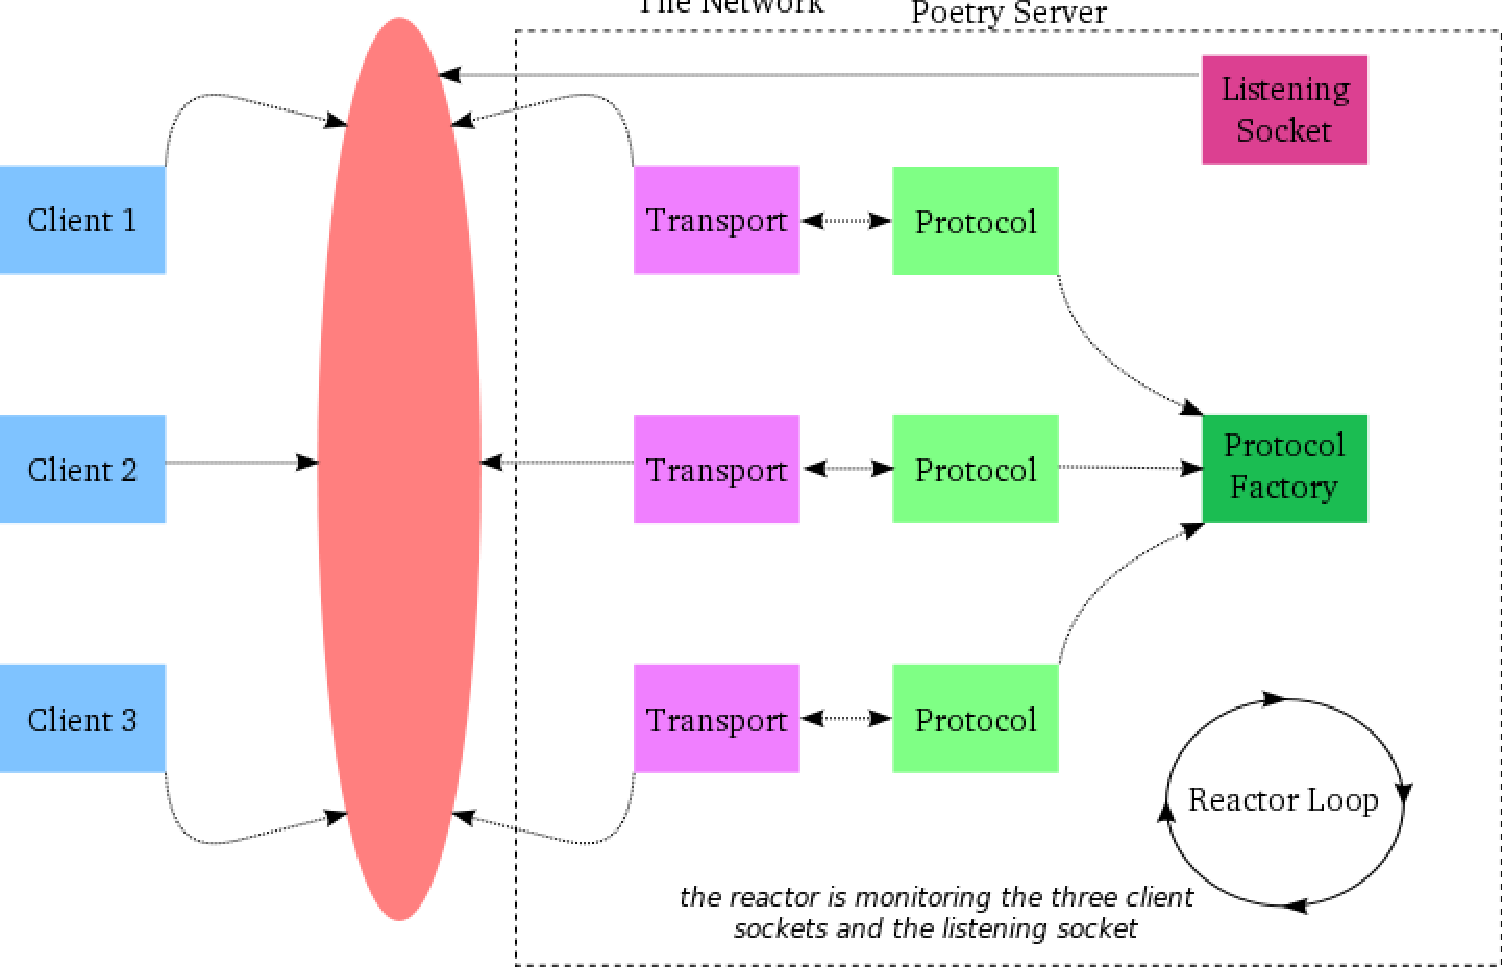
\includegraphics[width=0.7\textwidth]{images/server-1.pdf}
    \caption{Поэтический сервер в действии\label{fig:server-1}}
\end{center}
\end{figure}


На рисунке три клиента присоеденены к серверу. Каждый 
Transport представляет единственный клиентский сокет, и 
слушающий сокет делает в общей сложности 4 файловых дескриптора 
для мониторящего цикла операций ввода-вывода на  
основе select. Когда клиент отсоединяется, связанный с ним 
Transport и PoetryProtocol будет разыменован и утилизирован 
сборщиком мусора (предполагая, что мы не запрятали ссылку 
где-нибудь на один из них, нам не нужно 
предупреждать утечки памяти). PoetryFactory, между тем, не будет 
завершаться до тех пор пока мы будем слушать новые соединения, 
то есть, для нашего поэтического сервера, он будет висеть всегда. 


Клиентские сокеты и связанные с ними Python объекты не будут жить 
долго, если поэма, которую мы обслуживаем, относительно короткая. 
Но, с огромной поэмой и с относительно занятым сервером, мы могли 
бы оборваться из-за сотни или тысячи одновременных 
клиентов. И тут нет проблем, поскольку Twisted не имеет 
встроенных ограничений на количество соединений, которыми он 
может управлять. Конечно же, если вы увеличите нагрузку на 
любой сервер, то с какого-то момента, вы обнаружите, что 
сервер не может поддерживать такую нагрузку или, будет 
достигнуто внутреннее ограничение операционной системы. Для 
высоко-нагруженных серверов нужно тщательно измерять и тестировать пределльную нагрузку.


Twisted также не налагает ограничений на количество портов, 
которые вы можете слушать. Фактически, единственный Twisted процесс 
может слушать десятки портов и предоставлять различные сервисы на 
каждый (используя различные Factory-классы для каждого listenTCP вызова). 
И, при тщательном дизайне, решение, о том предоставлять ли несколько сервисов 
одним Twisted процессом или несколькими, 
потенциально можно отложить до этапа выкладки.


Есть несколько вещей, которые пропущены в нашем сервере. 
Прежде всего, он не создает никаких логов, которые 
могли бы помочь отладить проблемы или проанализировать 
наш сетевой трафик. Более того, сервер не запущен как 
демон, что делает его уязвимом в смысле завершения, 
при случайном нажатии Ctrl-C (или просто выхода из системы). 
Мы исправим эти две проблемы в следующей главе, но сначала, в 
главе 12, мы напишем еще один сервер, выполняющий 
поэтическое преобразование.


\subsection{Упражнения}

\begin{enumerate}

\item Напишите асинхронный поэтический сервер без 
использования Twisted, подобно тому, который мы сделали для 
клиента в главе 2. Заметьте, что слушающие сокеты нужно 
мониторить для чтения и, ``читабельность'' слушающего сокета 
означает, что мы можем принимать новый клиентский сокет.

\item Напишите высокоуровневую версию поэтического сервера 
``медленный сервер'' с использованием Twisted, 
используя callLater или \newline LoopingCall, 
для создания нескольких вызовов к 
transport.write(). Добавьте опции  \textit{\symbol{45}\symbol{45}num-bytes} и 
\textit{\symbol{45}\symbol{45}delay}  
в строку запуска, поддерживаемые блокирующим сервером. Не 
забудьте про случай, когда сервер отсоединяется до того, как 
получена вся поэма.

\item Расширьте высокоуровневый Twisted сервер так, чтобы он мог 
обслуживать несколько поэм (на различных портах).

\item Какие есть причины делать обслуживание нескольких сервисов в 
одном и том же Twisted процессе? Какие есть причины так не делать?

\end{enumerate}

